\begin{flushright} {\tiny {\color{gray} python\_codes/fieldstone\_00/text.tex}} \end{flushright}


%--------------------------------------------
\subsection*{The node layout}

Let us start in one dimension. We wish to generate a 
set of $N$ discrete and equidistant $x$ coordinates 
between $0$ and $L_x$:

\begin{center}
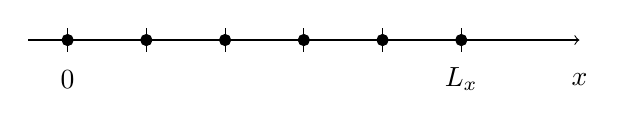
\begin{tikzpicture}
%\draw[fill=gray!23,gray!23](0,0) rectangle (8,2);
%\draw[step=0.5cm,gray,very thin] (0,0) grid (8,2); %background grid
\draw [->] (0.5,1) -- (7.5,1);
\draw[-] (1,0.85)--(1,1.15);
\draw[-] (2,0.85)--(2,1.15);
\draw[-] (3,0.85)--(3,1.15);
\draw[-] (4,0.85)--(4,1.15);
\draw[-] (5,0.85)--(5,1.15);
\draw[-] (6,0.85)--(6,1.15);
\node[] at (1,0.5) {$0$};
\node[] at (6,0.5) {$L_x$};
\node[] at (7.5,0.5) {$x$};
\draw[black,fill=black] (1,1)   circle (2pt);
\draw[black,fill=black] (2,1)   circle (2pt);
\draw[black,fill=black] (3,1)   circle (2pt);
\draw[black,fill=black] (4,1)   circle (2pt);
\draw[black,fill=black] (5,1)   circle (2pt);
\draw[black,fill=black] (6,1)   circle (2pt);
\end{tikzpicture}
\end{center}

\noindent
The distance between two consecutive coordinates is 
\[
h = \frac{L_x}{N-1}
\]
This simply translates as follows in Python:
\begin{lstlisting}
N=10
Lx=1
h=Lx/(N-1)
for i in range(0,N):
    print(i*h)
\end{lstlisting}

Since $i$ ranges from 0 to $N-1$ (because ... python!) the generated values go from 0 to $L_x$. 
Obviously I am doing this because I later wish to reuse these coordinates 
so I also wish to store them in an array.
I therefore need to declare and array of size $N$ which will 
contain all $N$ coordinates:
\begin{lstlisting}
import numpy as np
N=10
Lx=1
h=Lx/(N-1)
x=np.zeros(NV,dtype=np.float64)
for i in range(0,N):
    x[i]=i*h
\end{lstlisting}

What if now I wished the $N$ nodes (i.e. the coordinates of all points) to be placed between two arbitrary coordinates $x_{min}$ and $x_{max}$?

\begin{center}
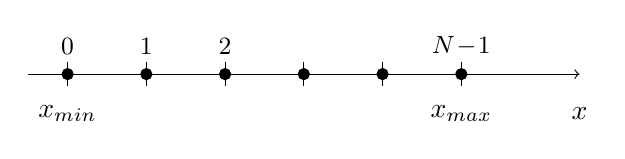
\begin{tikzpicture}
%\draw[fill=gray!23,gray!23](0,0) rectangle (8,2);
%\draw[step=0.5cm,gray,very thin] (0,0) grid (8,2); %background grid
\draw [->] (0.5,1) -- (7.5,1);
\draw[-] (1,0.85)--(1,1.15);
\draw[-] (2,0.85)--(2,1.15);
\draw[-] (3,0.85)--(3,1.15);
\draw[-] (4,0.85)--(4,1.15);
\draw[-] (5,0.85)--(5,1.15);
\draw[-] (6,0.85)--(6,1.15);
\node[] at (1,0.5) {$x_{min}$};
\node[] at (6,0.5) {$x_{max}$};
\node[] at (7.5,0.5) {$x$};
\draw[black,fill=black] (1,1)   circle (2pt);
\draw[black,fill=black] (2,1)   circle (2pt);
\draw[black,fill=black] (3,1)   circle (2pt);
\draw[black,fill=black] (4,1)   circle (2pt);
\draw[black,fill=black] (5,1)   circle (2pt);
\draw[black,fill=black] (6,1)   circle (2pt);
\node[] at (1,1.35) {\small 0};
\node[] at (2,1.35) {\small 1};
\node[] at (3,1.35) {\small 2};
\node[] at (6,1.35) {\small $N\!-\!1$};
\end{tikzpicture}
\end{center}

\noindent In this case the length of the domain is $L_x=x_{max}-x_{min}$, and the above code becomes:
\begin{lstlisting}
import numpy as np
N=10
xmin=-4
xmax=3
h=(xmax-xmin)/(N-1)
x=np.zeros(N,dtype=np.float64)
for i in range(0,N):
    x[i]=xmin+i*h
\end{lstlisting}
Note the presence of $x_{min}$ in the last line! 

\vspace{.8cm}

Unfortunately the world is definitely not one-dimensional, so 
I may want to build a two-dimensional grid spanning the domain 
$[0,L_x]\times[0,L_y]$ as depicted here:



\begin{center}
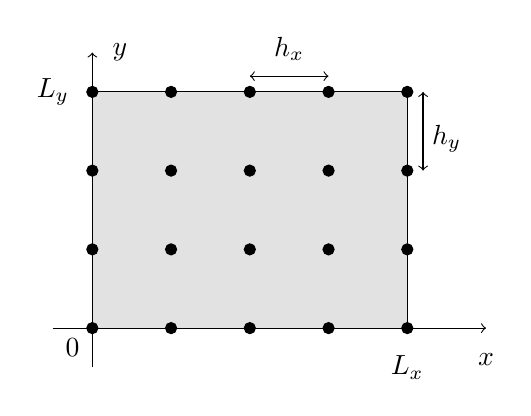
\begin{tikzpicture}
\draw[fill=gray!23,gray!23](1,1) rectangle (5,4);
%\draw[step=0.5cm,gray,very thin] (0,0) grid (7,5); 
\draw [->] (0.5,1) -- (6,1);
\draw [->] (1,0.5) -- (1,4.5);
\node[] at (0.75,0.75) {$0$};
\node[] at (5,0.5) {$L_x$};
\node[] at (0.5,4) {$L_y$};
\node[] at (6,0.6) {$x$};
\node[] at (1.35,4.5) {$y$};
\draw[-] (1,1)--(5,1)--(5,4)--(1,4)--cycle;
\draw[black,fill=black] (1,1)   circle (2pt);
\draw[black,fill=black] (2,1)   circle (2pt);
\draw[black,fill=black] (3,1)   circle (2pt);
\draw[black,fill=black] (4,1)   circle (2pt);
\draw[black,fill=black] (5,1)   circle (2pt);
\draw[black,fill=black] (1,2)   circle (2pt);
\draw[black,fill=black] (2,2)   circle (2pt);
\draw[black,fill=black] (3,2)   circle (2pt);
\draw[black,fill=black] (4,2)   circle (2pt);
\draw[black,fill=black] (5,2)   circle (2pt);
\draw[black,fill=black] (1,3)   circle (2pt);
\draw[black,fill=black] (2,3)   circle (2pt);
\draw[black,fill=black] (3,3)   circle (2pt);
\draw[black,fill=black] (4,3)   circle (2pt);
\draw[black,fill=black] (5,3)   circle (2pt);
\draw[black,fill=black] (1,4)   circle (2pt);
\draw[black,fill=black] (2,4)   circle (2pt);
\draw[black,fill=black] (3,4)   circle (2pt);
\draw[black,fill=black] (4,4)   circle (2pt);
\draw[black,fill=black] (5,4)   circle (2pt);
\draw[<->] (5.2,3)--(5.2,4);
\draw[<->] (3,4.2)--(4,4.2);
\node[] at (3.5,4.55) {$h_x$};
\node[] at (5.5,3.4) {$h_y$};
\end{tikzpicture}
\end{center}

\noindent There are now $N=N_x \times N_y$ nodes in the mesh, 
and we need to define the mesh spacing in both the $x$ and $y$
direction:
\[
h_x = \frac{L_x}{N_x-1}
\qquad\qquad
h_y = \frac{L_y}{N_y-1}
\]
From our experience with the 1D case, it seems logical to 
resort to a double for loop, one in the $x$ direction, 
one in the $y$ direction. 
However we must now make a decision as to which loop is inside the other (inner loop vs. outer loop). In essence, I must decide between 
\begin{lstlisting}
#approach 1
for i in range(0,Nx):
    for j in range(0,Ny):
\end{lstlisting}
and
\begin{lstlisting}
#approach 2
for j in range(0,Ny):
    for i in range(0,Nx):
\end{lstlisting}
As it turns out, I need not decide, both options are equally valid as we will see.
I now fix $N_x=4$ and $N_y=3$ so that the mesh contains 12 nodes:

\begin{center}
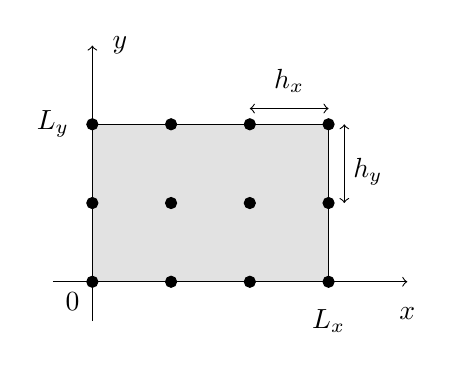
\begin{tikzpicture}
\draw[fill=gray!23,gray!23](1,1) rectangle (4,3);
%\draw[step=0.5cm,gray,very thin] (0,0) grid (7,5); 
\draw [->] (0.5,1) -- (5,1);
\draw [->] (1,0.5) -- (1,4);
\node[] at (0.75,0.75) {$0$};
\node[] at (4,0.5) {$L_x$};
\node[] at (0.5,3) {$L_y$};
\node[] at (5,0.6) {$x$};
\node[] at (1.35,4) {$y$};
\draw[-] (1,1)--(4,1)--(4,3)--(1,3)--cycle;
\draw[black,fill=black] (1,1)   circle (2pt);
\draw[black,fill=black] (2,1)   circle (2pt);
\draw[black,fill=black] (3,1)   circle (2pt);
\draw[black,fill=black] (4,1)   circle (2pt);
\draw[black,fill=black] (1,2)   circle (2pt);
\draw[black,fill=black] (2,2)   circle (2pt);
\draw[black,fill=black] (3,2)   circle (2pt);
\draw[black,fill=black] (4,2)   circle (2pt);
\draw[black,fill=black] (1,3)   circle (2pt);
\draw[black,fill=black] (2,3)   circle (2pt);
\draw[black,fill=black] (3,3)   circle (2pt);
\draw[black,fill=black] (4,3)   circle (2pt);
\draw[<->] (4.2,2)--(4.2,3);
\draw[<->] (3,3.2)--(4,3.2);
\node[] at (3.5,3.55) {$h_x$};
\node[] at (4.5,2.4) {$h_y$};
\end{tikzpicture}
\end{center}

\noindent Looking at approach \#1, I can include a print statement inside the loops as follows:
\begin{lstlisting}
#option 1
Nx=4
Ny=3
for i in range(0,Nx):
    for j in range(0,Ny):
        print('i=',i,'; j=',j)
\end{lstlisting}
If I was to run this code it would display (I first exhaust the $j$ values from the inner most loop before I switch to a different $i$ value):
\begin{lstlisting}
i= 0  ; j= 0
i= 0  ; j= 1
i= 0  ; j= 2
i= 1  ; j= 0
i= 1  ; j= 1
i= 1  ; j= 2
i= 2  ; j= 0
i= 2  ; j= 1
i= 2  ; j= 2
i= 3  ; j= 0
i= 3  ; j= 1
i= 3  ; j= 2
\end{lstlisting}
This means that the code is going through the nodes in the following order:
\begin{center}
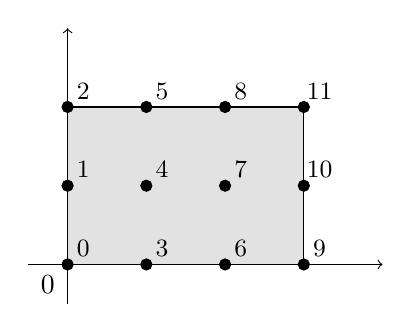
\begin{tikzpicture}
\draw[fill=gray!23,gray!23](1,1) rectangle (4,3);
%\draw[step=0.5cm,gray,very thin] (0,0) grid (7,5); 
\draw [->] (0.5,1) -- (5,1);
\draw [->] (1,0.5) -- (1,4);
\node[] at (0.75,0.75) {$0$};
\draw[-] (1,1)--(4,1)--(4,3)--(1,3)--cycle;
\draw[black,fill=black] (1,1)   circle (2pt);
\draw[black,fill=black] (2,1)   circle (2pt);
\draw[black,fill=black] (3,1)   circle (2pt);
\draw[black,fill=black] (4,1)   circle (2pt);
\draw[black,fill=black] (1,2)   circle (2pt);
\draw[black,fill=black] (2,2)   circle (2pt);
\draw[black,fill=black] (3,2)   circle (2pt);
\draw[black,fill=black] (4,2)   circle (2pt);
\draw[black,fill=black] (1,3)   circle (2pt);
\draw[black,fill=black] (2,3)   circle (2pt);
\draw[black,fill=black] (3,3)   circle (2pt);
\draw[black,fill=black] (4,3)   circle (2pt);
\node[] at (1.2,1.2) {\small $0$};
\node[] at (2.2,1.2) {\small $3$};
\node[] at (3.2,1.2) {\small $6$};
\node[] at (4.2,1.2) {\small $9$};
\node[] at (1.2,2.2) {\small $1$};
\node[] at (2.2,2.2) {\small $4$};
\node[] at (3.2,2.2) {\small $7$};
\node[] at (4.2,2.2) {\small $10$};
\node[] at (1.2,3.2) {\small $2$};
\node[] at (2.2,3.2) {\small $5$};
\node[] at (3.2,3.2) {\small $8$};
\node[] at (4.2,3.2) {\small $11$};
\end{tikzpicture}
\end{center}



Turning now to approach \#2, the same print statement will now yield:
\begin{lstlisting}
i= 0 ; j= 0
i= 1 ; j= 0
i= 2 ; j= 0
i= 3 ; j= 0
i= 0 ; j= 1
i= 1 ; j= 1
i= 2 ; j= 1
i= 3 ; j= 1
i= 0 ; j= 2
i= 1 ; j= 2
i= 2 ; j= 2
i= 3 ; j= 2
\end{lstlisting}
and this corresponds then to the following order: 
\begin{center}
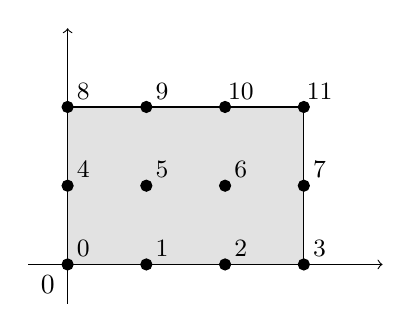
\begin{tikzpicture}
\draw[fill=gray!23,gray!23](1,1) rectangle (4,3);
%\draw[step=0.5cm,gray,very thin] (0,0) grid (7,5); 
\draw [->] (0.5,1) -- (5,1);
\draw [->] (1,0.5) -- (1,4);
\node[] at (0.75,0.75) {$0$};
\draw[-] (1,1)--(4,1)--(4,3)--(1,3)--cycle;
\draw[black,fill=black] (1,1)   circle (2pt);
\draw[black,fill=black] (2,1)   circle (2pt);
\draw[black,fill=black] (3,1)   circle (2pt);
\draw[black,fill=black] (4,1)   circle (2pt);
\draw[black,fill=black] (1,2)   circle (2pt);
\draw[black,fill=black] (2,2)   circle (2pt);
\draw[black,fill=black] (3,2)   circle (2pt);
\draw[black,fill=black] (4,2)   circle (2pt);
\draw[black,fill=black] (1,3)   circle (2pt);
\draw[black,fill=black] (2,3)   circle (2pt);
\draw[black,fill=black] (3,3)   circle (2pt);
\draw[black,fill=black] (4,3)   circle (2pt);
\node[] at (1.2,1.2) {\small $0$};
\node[] at (2.2,1.2) {\small $1$};
\node[] at (3.2,1.2) {\small $2$};
\node[] at (4.2,1.2) {\small $3$};
\node[] at (1.2,2.2) {\small $4$};
\node[] at (2.2,2.2) {\small $5$};
\node[] at (3.2,2.2) {\small $6$};
\node[] at (4.2,2.2) {\small $7$};
\node[] at (1.2,3.2) {\small $8$};
\node[] at (2.2,3.2) {\small $9$};
\node[] at (3.2,3.2) {\small $10$};
\node[] at (4.2,3.2) {\small $11$};
\end{tikzpicture}
\end{center}

\noindent In the end, we see that both approaches yield a valid 
numbering scheme, one is 'lines first' , the other 'columns first'.

In what follows I focus on approach \#2, only because it seems more 'natural' to me than the other one (it goes from left to right, then bottom to top). 
Our proto-code then looks like this:
\begin{lstlisting}
Lx=10
Ly=8
Nx=4
Ny=3
N=Nx*Ny
hx=Lx/(Nx-1)
hy=Ly/(Ny-1)
x=np.zeros(N,dtype=np.float64)
y=np.zeros(N,dtype=np.float64)
for j in range(0,Ny):
    for i in range(0,Nx):
        x[?]=i*hx
        y[?]=j*hy
\end{lstlisting}
Note that I have left two question marks. One may want to replace these by $i$ and $j$, 
following our experience in the 1D case. However, remember that $i$ ($j$) ranges between 
$0$ and $N_x-1=3$ ($0$ and $N_y-1=2$ respectively) but we need to assign and store the 
coordinates of all 12 nodes. 

So what should I write instead of question marks? Effectively, I need some form of counter 
so that every time the inner loop is executed the counter is incremented by one. 
When all $i,j$ combinations are exhausted this counter should have reached the 
last node. Such a counter can be implemented as follows:
\begin{lstlisting}
counter=0
for j in range(0,Ny):
    for i in range(0,Nx):
        print('counter=',counter,'i=',i,'; j=',j,j*Nx+i)
        counter+=1
\end{lstlisting}
It must be initialised to zero, and it is incremented $N_x \cdot N_y$ times.
Running this code would yield 
\begin{lstlisting}
counter=  0 i= 0 ; j= 0
counter=  1 i= 1 ; j= 0
counter=  2 i= 2 ; j= 0
counter=  3 i= 3 ; j= 0
counter=  4 i= 0 ; j= 1
counter=  5 i= 1 ; j= 1
counter=  6 i= 2 ; j= 1
counter=  7 i= 3 ; j= 1
counter=  8 i= 0 ; j= 2
counter=  9 i= 1 ; j= 2
counter= 10 i= 2 ; j= 2
counter= 11 i= 3 ; j= 2
\end{lstlisting}
We see that the counter takes all 12 values between 0 and 11, so it is the index I am looking for. Finally, the 2D code (or approach \#2) looks like:
\begin{lstlisting}
Lx=10
Ly=8
Nx=4
Ny=3
N=Nx*Ny
hx=Lx/(Nx-1)
hy=Ly/(Ny-1)
x=np.zeros(N,dtype=np.float64)
y=np.zeros(N,dtype=np.float64)
counter=0
for j in range(0,Ny):
    for i in range(0,Nx):
        x[counter]=i*hx
        y[counter]=j*hy
        counter+=1
\end{lstlisting}
It is trivial to verify that one can swap the two lines with the 'for' statements to obtain the approach \#1 version of the code.

Before I move to the three-dimensional case, I wish to mention a slightly different 
approach than the 'counter' one. 
Looking back at the numbering generated by approach \#2, it is easy to see that the node number (i.e. a value between 0 and 11)
can be also computed with $j\cdot N_x+i$. You can indeed verify that this expression yields the same values as the counter here above for all the $i,j$ combinations. However one must realise that this formula is not valid for approach \#1. The code then becomes:
\begin{lstlisting}
Lx=10
Ly=8
Nx=4
Ny=3
N=Nx*Ny
hx=Lx/(Nx-1)
hy=Ly/(Ny-1)
x=np.zeros(N,dtype=np.float64)
y=np.zeros(N,dtype=np.float64)
for j in range(0,Ny):
    for i in range(0,Nx):
        x[j*Nx+i]=i*hx
        y[j*Nx+i]=j*hy
\end{lstlisting}

Also, if the domain is not $[0,L_x]\times[0,L_y]$ but
$[x_{min},x_{max}]\times[y_{min},y_{max}]$, the code becomes
\begin{lstlisting}
xmin=-3
xmax=5
ymin=-1
ymax=4
Nx=4
Ny=3
N=Nx*Ny
hx=(xmax-xmin)/(Nx-1)
hy=(ymax-ymin)/(Ny-1)
x=np.zeros(N,dtype=np.float64)
y=np.zeros(N,dtype=np.float64)
for j in range(0,Ny):
    for i in range(0,Nx):
        x[j*Nx+i]=xmin+i*hx
        y[j*Nx+i]=ymin+j*hy
\end{lstlisting}

\vspace{.8cm}

Extending the codes above to three-dimensions is rather trivial, especially when the counter approach 
is used. One must simply be aware of the order of the loops (there are 3\! =6 approaches).
\begin{lstlisting}
xmin=-3
xmax=5
ymin=-1
ymax=4
zmin=1
zmax=6
Nx=4
Ny=3
Nz=5
N=Nx*Ny*Nz
hx=(xmax-xmin)/(Nx-1)
hy=(ymax-ymin)/(Ny-1)
hz=(zmax-zmin)/(Nz-1)
x=np.zeros(N,dtype=np.float64)
y=np.zeros(N,dtype=np.float64)
z=np.zeros(N,dtype=np.float64)
counter
for k in range(0,Nz):
    for j in range(0,Ny):
        for i in range(0,Nx):
            x[counter]=xmin+i*hx
            y[counter]=ymin+j*hy
            z[counter]=zmin+k*hz
            counter+=1
\end{lstlisting}
You will find near identical codes in (for example) Stone 1 and 10.

\vspace{.8cm}

In some cases, we wish to store the coordinates of the mesh nodes because the nodes 
make a regular grid of quadrilaterals on which ODEs or PDEs will be solved:

\begin{center}
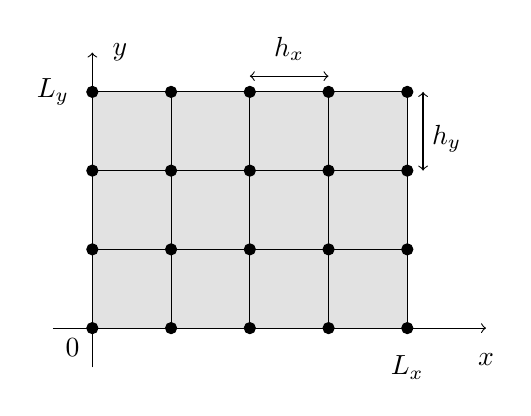
\begin{tikzpicture}
\draw[fill=gray!23,gray!23](1,1) rectangle (5,4);
%\draw[step=0.5cm,gray,very thin] (0,0) grid (7,5); 
\draw [->] (0.5,1) -- (6,1);
\draw [->] (1,0.5) -- (1,4.5);
\node[] at (0.75,0.75) {$0$};
\node[] at (5,0.5) {$L_x$};
\node[] at (0.5,4) {$L_y$};
\node[] at (6,0.6) {$x$};
\node[] at (1.35,4.5) {$y$};
\draw[-] (1,1)--(5,1)--(5,4)--(1,4)--cycle;
\draw[-] (1,2)--(5,2);
\draw[-] (1,3)--(5,3);
\draw[-] (2,1)--(2,4);
\draw[-] (3,1)--(3,4);
\draw[-] (4,1)--(4,4);
\draw[black,fill=black] (1,1)   circle (2pt);
\draw[black,fill=black] (2,1)   circle (2pt);
\draw[black,fill=black] (3,1)   circle (2pt);
\draw[black,fill=black] (4,1)   circle (2pt);
\draw[black,fill=black] (5,1)   circle (2pt);
\draw[black,fill=black] (1,2)   circle (2pt);
\draw[black,fill=black] (2,2)   circle (2pt);
\draw[black,fill=black] (3,2)   circle (2pt);
\draw[black,fill=black] (4,2)   circle (2pt);
\draw[black,fill=black] (5,2)   circle (2pt);
\draw[black,fill=black] (1,3)   circle (2pt);
\draw[black,fill=black] (2,3)   circle (2pt);
\draw[black,fill=black] (3,3)   circle (2pt);
\draw[black,fill=black] (4,3)   circle (2pt);
\draw[black,fill=black] (5,3)   circle (2pt);
\draw[black,fill=black] (1,4)   circle (2pt);
\draw[black,fill=black] (2,4)   circle (2pt);
\draw[black,fill=black] (3,4)   circle (2pt);
\draw[black,fill=black] (4,4)   circle (2pt);
\draw[black,fill=black] (5,4)   circle (2pt);
\draw[<->] (5.2,3)--(5.2,4);
\draw[<->] (3,4.2)--(4,4.2);
\node[] at (3.5,4.55) {$h_x$};
\node[] at (5.5,3.4) {$h_y$};
\end{tikzpicture}
\end{center}

There are $N_x$ nodes in the $x$ direction but only $N_x-1$ cells/elements\footnote{Because of my 
bias towards the Finite Element Method, I will refer to these as elements.}. 
Likewise there are $N_y$ nodes in the $y$ direction but only $N_y-1$ cells/elements.
In total there are $N_e=(N_x-1)(N_y-1)$ elements. 
As for the cell center nodes, we must adopt a systematic way of numbering them. 
If I keep using approach \#2 for the nodes, the following numbering of 
{\color{teal}elements} seems natural:

\begin{center}
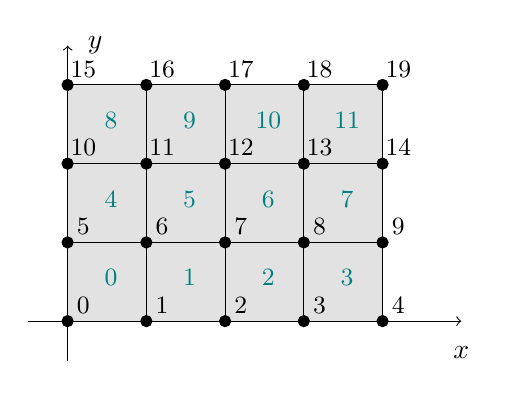
\begin{tikzpicture}
\draw[fill=gray!23,gray!23](1,1) rectangle (5,4);
%\draw[step=0.5cm,gray,very thin] (0,0) grid (7,5); 
\draw [->] (0.5,1) -- (6,1);
\draw [->] (1,0.5) -- (1,4.5);
\node[] at (6,0.6) {$x$};
\node[] at (1.35,4.5) {$y$};
\draw[-] (1,1)--(5,1)--(5,4)--(1,4)--cycle;
\draw[-] (1,2)--(5,2);
\draw[-] (1,3)--(5,3);
\draw[-] (2,1)--(2,4);
\draw[-] (3,1)--(3,4);
\draw[-] (4,1)--(4,4);
\draw[black,fill=black] (1,1)   circle (2pt);
\draw[black,fill=black] (2,1)   circle (2pt);
\draw[black,fill=black] (3,1)   circle (2pt);
\draw[black,fill=black] (4,1)   circle (2pt);
\draw[black,fill=black] (5,1)   circle (2pt);
\draw[black,fill=black] (1,2)   circle (2pt);
\draw[black,fill=black] (2,2)   circle (2pt);
\draw[black,fill=black] (3,2)   circle (2pt);
\draw[black,fill=black] (4,2)   circle (2pt);
\draw[black,fill=black] (5,2)   circle (2pt);
\draw[black,fill=black] (1,3)   circle (2pt);
\draw[black,fill=black] (2,3)   circle (2pt);
\draw[black,fill=black] (3,3)   circle (2pt);
\draw[black,fill=black] (4,3)   circle (2pt);
\draw[black,fill=black] (5,3)   circle (2pt);
\draw[black,fill=black] (1,4)   circle (2pt);
\draw[black,fill=black] (2,4)   circle (2pt);
\draw[black,fill=black] (3,4)   circle (2pt);
\draw[black,fill=black] (4,4)   circle (2pt);
\draw[black,fill=black] (5,4)   circle (2pt);
\node[] at (1.2,1.2) {\small $0$};
\node[] at (2.2,1.2) {\small $1$};
\node[] at (3.2,1.2) {\small $2$};
\node[] at (4.2,1.2) {\small $3$};
\node[] at (5.2,1.2) {\small $4$};
\node[] at (1.2,2.2) {\small $5$};
\node[] at (2.2,2.2) {\small $6$};
\node[] at (3.2,2.2) {\small $7$};
\node[] at (4.2,2.2) {\small $8$};
\node[] at (5.2,2.2) {\small $9$};
\node[] at (1.2,3.2) {\small $10$};
\node[] at (2.2,3.2) {\small $11$};
\node[] at (3.2,3.2) {\small $12$};
\node[] at (4.2,3.2) {\small $13$};
\node[] at (5.2,3.2) {\small $14$};
\node[] at (1.2,4.2) {\small $15$};
\node[] at (2.2,4.2) {\small $16$};
\node[] at (3.2,4.2) {\small $17$};
\node[] at (4.2,4.2) {\small $18$};
\node[] at (5.2,4.2) {\small $19$};
\node[] at (1.55,1.55) {\color{teal} \small $0$};
\node[] at (2.55,1.55) {\color{teal} \small $1$};
\node[] at (3.55,1.55) {\color{teal} \small $2$};
\node[] at (4.55,1.55) {\color{teal} \small $3$};
\node[] at (1.55,2.55) {\color{teal} \small $4$};
\node[] at (2.55,2.55) {\color{teal} \small $5$};
\node[] at (3.55,2.55) {\color{teal} \small $6$};
\node[] at (4.55,2.55) {\color{teal} \small $7$};
\node[] at (1.55,3.55) {\color{teal} \small $8$};
\node[] at (2.55,3.55) {\color{teal} \small $9$};
\node[] at (3.55,3.55) {\color{teal} \small $10$};
\node[] at (4.55,3.55) {\color{teal} \small $11$};
\end{tikzpicture}
\end{center}

In some applications we want to also store the coordinates of the center of all cells, i.e. the $N_e$ coordinates of {\color{teal} these} points:

\begin{center}
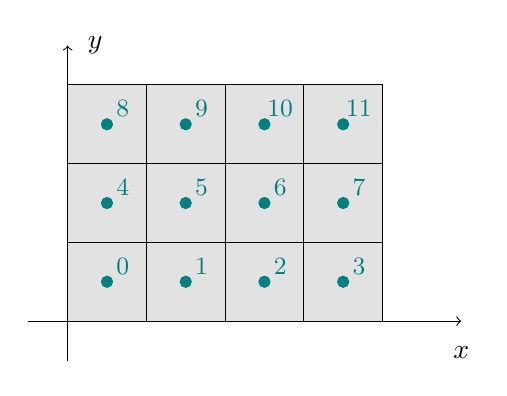
\begin{tikzpicture}
\draw[fill=gray!23,gray!23](1,1) rectangle (5,4);
%\draw[step=0.5cm,gray,very thin] (0,0) grid (7,5); 
\draw [->] (0.5,1) -- (6,1);
\draw [->] (1,0.5) -- (1,4.5);
\node[] at (6,0.6) {$x$};
\node[] at (1.35,4.5) {$y$};
\draw[-] (1,1)--(5,1)--(5,4)--(1,4)--cycle;
\draw[-] (1,2)--(5,2);
\draw[-] (1,3)--(5,3);
\draw[-] (2,1)--(2,4);
\draw[-] (3,1)--(3,4);
\draw[-] (4,1)--(4,4);
\draw[black,fill=black,color=teal] (1.5,1.5)   circle (2pt);
\draw[black,fill=black,color=teal] (2.5,1.5)   circle (2pt);
\draw[black,fill=black,color=teal] (3.5,1.5)   circle (2pt);
\draw[black,fill=black,color=teal] (4.5,1.5)   circle (2pt);
\draw[black,fill=black,color=teal] (1.5,2.5)   circle (2pt);
\draw[black,fill=black,color=teal] (2.5,2.5)   circle (2pt);
\draw[black,fill=black,color=teal] (3.5,2.5)   circle (2pt);
\draw[black,fill=black,color=teal] (4.5,2.5)   circle (2pt);
\draw[black,fill=black,color=teal] (1.5,3.5)   circle (2pt);
\draw[black,fill=black,color=teal] (2.5,3.5)   circle (2pt);
\draw[black,fill=black,color=teal] (3.5,3.5)   circle (2pt);
\draw[black,fill=black,color=teal] (4.5,3.5)   circle (2pt);
\node[] at (1.7,1.7) {\color{teal} \small $0$};
\node[] at (2.7,1.7) {\color{teal} \small $1$};
\node[] at (3.7,1.7) {\color{teal} \small $2$};
\node[] at (4.7,1.7) {\color{teal} \small $3$};
\node[] at (1.7,2.7) {\color{teal} \small $4$};
\node[] at (2.7,2.7) {\color{teal} \small $5$};
\node[] at (3.7,2.7) {\color{teal} \small $6$};
\node[] at (4.7,2.7) {\color{teal} \small $7$};
\node[] at (1.7,3.7) {\color{teal} \small $8$};
\node[] at (2.7,3.7) {\color{teal} \small $9$};
\node[] at (3.7,3.7) {\color{teal} \small $10$};
\node[] at (4.7,3.7) {\color{teal} \small $11$};
\end{tikzpicture}
\end{center}
Given this numbering these points form a regular grid:
\begin{center}
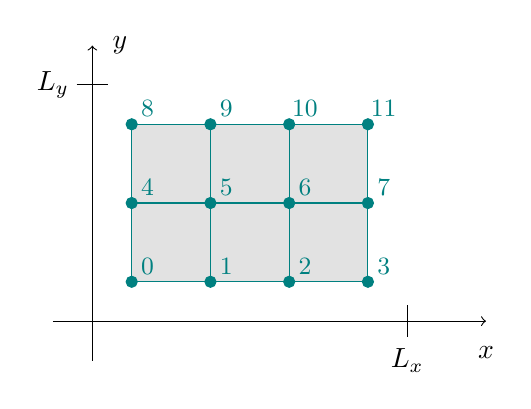
\begin{tikzpicture}
\draw[fill=gray!23,gray!23](1.5,1.5) rectangle (4.5,3.5);
%\draw[step=0.5cm,gray,very thin] (0,0) grid (7,5); 
\draw [->] (0.5,1) -- (6,1);
\draw [->] (1,0.5) -- (1,4.5);
\node[] at (6,0.6) {$x$};
\node[] at (1.35,4.5) {$y$};
\draw[-,teal] (1.5,1.5)--(4.5,1.5)--(4.5,3.5)--(1.5,3.5)--cycle;
\draw[-,teal] (1.5,2.5)--(4.5,2.5);
\draw[-,teal] (2.5,1.5)--(2.5,3.5);
\draw[-,teal] (3.5,1.5)--(3.5,3.5);
\draw[black,fill=black,color=teal] (1.5,1.5)   circle (2pt);
\draw[black,fill=black,color=teal] (2.5,1.5)   circle (2pt);
\draw[black,fill=black,color=teal] (3.5,1.5)   circle (2pt);
\draw[black,fill=black,color=teal] (4.5,1.5)   circle (2pt);
\draw[black,fill=black,color=teal] (1.5,2.5)   circle (2pt);
\draw[black,fill=black,color=teal] (2.5,2.5)   circle (2pt);
\draw[black,fill=black,color=teal] (3.5,2.5)   circle (2pt);
\draw[black,fill=black,color=teal] (4.5,2.5)   circle (2pt);
\draw[black,fill=black,color=teal] (1.5,3.5)   circle (2pt);
\draw[black,fill=black,color=teal] (2.5,3.5)   circle (2pt);
\draw[black,fill=black,color=teal] (3.5,3.5)   circle (2pt);
\draw[black,fill=black,color=teal] (4.5,3.5)   circle (2pt);
\node[] at (1.7,1.7) {\color{teal} \small $0$};
\node[] at (2.7,1.7) {\color{teal} \small $1$};
\node[] at (3.7,1.7) {\color{teal} \small $2$};
\node[] at (4.7,1.7) {\color{teal} \small $3$};
\node[] at (1.7,2.7) {\color{teal} \small $4$};
\node[] at (2.7,2.7) {\color{teal} \small $5$};
\node[] at (3.7,2.7) {\color{teal} \small $6$};
\node[] at (4.7,2.7) {\color{teal} \small $7$};
\node[] at (1.7,3.7) {\color{teal} \small $8$};
\node[] at (2.7,3.7) {\color{teal} \small $9$};
\node[] at (3.7,3.7) {\color{teal} \small $10$};
\node[] at (4.7,3.7) {\color{teal} \small $11$};
\draw[-] (5,0.8)--(5,1.2);
\draw[-] (0.8,4)--(1.2,4);
\node[] at (5,0.5) {$L_x$};
\node[] at (0.5,4) {$L_y$};
\end{tikzpicture}
\end{center}
This 'new' domain is bound by $x'_{min}=h_x/2$, $x'_{max}=L_x-h_x/2$ in 
the $x$ direction and $y'_{min}=h/2$, $y'_{max}=L_y-h_y/2$ in the $y$ direction. We note that the spacings $h_x$ and $h_y$ between the centers is the same as for the nodes. 
We store the coordinates $(x_c,y_c)$ of the cell centers in two arrays of length $N_e$ and the code is then simply

\begin{lstlisting}
Lx=9
Ly=7
Nx=4
Ny=3
N=Nx*Ny
hx=(xmax-xmin)/(Nx-1)
hy=(ymax-ymin)/(Ny-1)
#mesh nodes coordinates
x=np.zeros(N,dtype=np.float64)
y=np.zeros(N,dtype=np.float64)
counter=0
for j in range(0,Ny):
    for i in range(0,Nx):
        x[counter]=i*hx
        y[counter]=j*hy
        counter+=1
#cell centers coordinates
Ne=(Nx-1)*(Ny-1)
xc=np.zeros(Ne,dtype=np.float64)
yc=np.zeros(Ne,dtype=np.float64)
xmin=hx/2
xmax=Lx-hx/2
ymin=hy/2
ymax=Ly-hy/2
counter=0
for j in range(0,Ny-1):
    for i in range(0,Nx-1):
        xc[counter]=xmin+i*hx
        yc[counter]=ymin+j*hy
        counter+=1
\end{lstlisting}

%--------------------------------------------
\subsection*{The connectivity array}

Let us consider 3 points in a plane:
\begin{center}
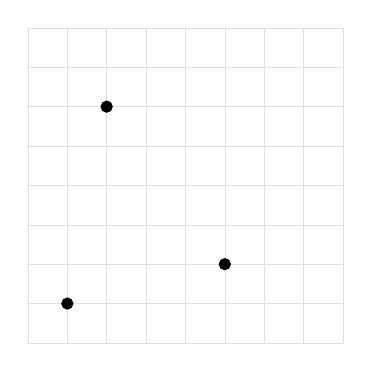
\begin{tikzpicture}
\draw[step=0.5cm,gray!25,very thin] (0.5,0.5) grid (4.5,4.5); 
\draw[black,fill=black] (1,1)   circle (2pt);
\draw[black,fill=black] (3,1.5)   circle (2pt);
\draw[black,fill=black] (1.5,3.5)   circle (2pt);
\end{tikzpicture}
\end{center}
Since they are not aligned they form a triangle:
\begin{center}
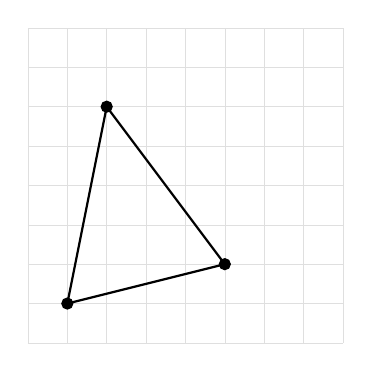
\begin{tikzpicture}
\draw[step=0.5cm,gray!25,very thin] (0.5,0.5) grid (4.5,4.5); 
\draw[black,fill=black] (1,1)   circle (2pt);
\draw[black,fill=black] (3,1.5)   circle (2pt);
\draw[black,fill=black] (1.5,3.5)   circle (2pt);
\draw[-,thick] (1,1)--(3,1.5)--(1.5,3.5)--cycle;
\end{tikzpicture}
\end{center}
When it comes to assigning these points an identity (or a number), I can arbitrarily assign them the following numbers:
\begin{center}
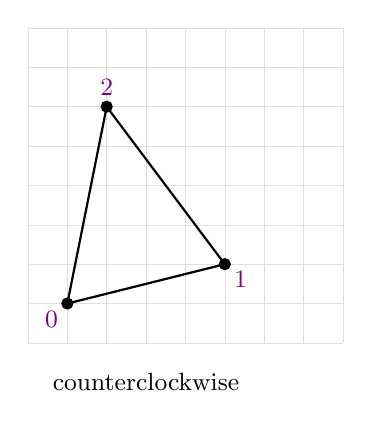
\begin{tikzpicture}
\draw[step=0.5cm,gray!25,very thin] (0.5,0.5) grid (4.5,4.5); 
\draw[black,fill=black] (1,1)   circle (2pt);
\draw[black,fill=black] (3,1.5)   circle (2pt);
\draw[black,fill=black] (1.5,3.5)   circle (2pt);
\draw[-,thick] (1,1)--(3,1.5)--(1.5,3.5)--cycle;
\node[] at (0.8,0.8) {\small \color{violet}0};
\node[] at (3.2,1.3) {\small \color{violet}1};
\node[] at (1.5,3.75) {\small \color{violet}2};
\node[] at (2,0) {\small counterclockwise};
\end{tikzpicture}
\end{center}
This triangle is then made of nodes {\color{violet}0}, 
{\color{violet}1}, and {\color{violet}2}.

Let us now add one more point in the plane as follows:
\begin{center}
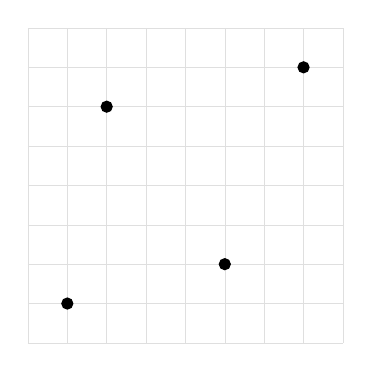
\begin{tikzpicture}
\draw[step=0.5cm,gray!25,very thin] (0.5,0.5) grid (4.5,4.5); 
\draw[black,fill=black] (1,1)   circle (2pt);
\draw[black,fill=black] (3,1.5)   circle (2pt);
\draw[black,fill=black] (1.5,3.5)   circle (2pt);
\draw[black,fill=black] (4,4)   circle (2pt);
\end{tikzpicture}
\end{center}
I will here number them as follows:
\begin{center}
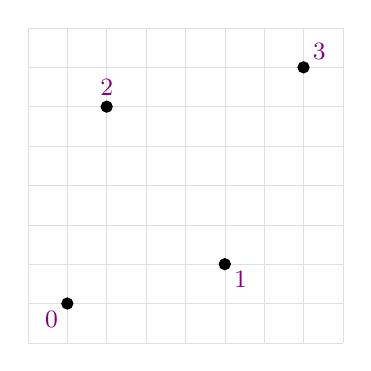
\begin{tikzpicture}
\draw[step=0.5cm,gray!25,very thin] (0.5,0.5) grid (4.5,4.5); 
\draw[black,fill=black] (1,1)   circle (2pt);
\draw[black,fill=black] (3,1.5)   circle (2pt);
\draw[black,fill=black] (1.5,3.5)   circle (2pt);
\draw[black,fill=black] (4,4)   circle (2pt);
\node[] at (0.8,0.8) {\small \color{violet}0};
\node[] at (3.2,1.3) {\small \color{violet}1};
\node[] at (1.5,3.75) {\small \color{violet}2};
\node[] at (4.2,4.2) {\small \color{violet}3};
\end{tikzpicture}
\end{center}

I can either decide to see them as the vertices of a quadrilateral, or
as the vertices of two triangles. However, there are two possibilities for the triangles:

\begin{center}
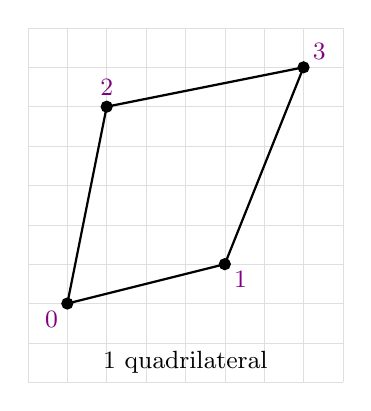
\begin{tikzpicture}
\draw[step=0.5cm,gray!25,very thin] (0.5,0) grid (4.5,4.5); 
\draw[black,fill=black] (1,1)   circle (2pt);
\draw[black,fill=black] (3,1.5)   circle (2pt);
\draw[black,fill=black] (1.5,3.5)   circle (2pt);
\draw[black,fill=black] (4,4)   circle (2pt);
\draw[-,thick] (1,1)--(3,1.5)--(4,4)--(1.5,3.5)--cycle;
\node[] at (0.8,0.8) {\small \color{violet}0};
\node[] at (3.2,1.3) {\small \color{violet}1};
\node[] at (1.5,3.75) {\small \color{violet}2};
\node[] at (4.2,4.2) {\small \color{violet}3};
\node[] at (2.5,0.25) {\small 1 quadrilateral};
\end{tikzpicture}
\hspace{1cm}
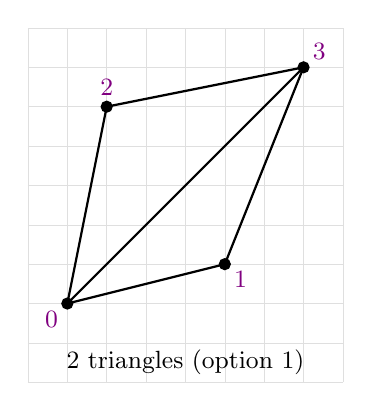
\begin{tikzpicture}
\draw[step=0.5cm,gray!25,very thin] (0.5,0) grid (4.5,4.5); 
\draw[black,fill=black] (1,1)   circle (2pt);
\draw[black,fill=black] (3,1.5)   circle (2pt);
\draw[black,fill=black] (1.5,3.5)   circle (2pt);
\draw[black,fill=black] (4,4)   circle (2pt);
\draw[-,thick] (1,1)--(3,1.5)--(4,4)--(1.5,3.5)--cycle;
\draw[-,thick] (1,1)--(4,4);
\node[] at (0.8,0.8) {\small \color{violet}0};
\node[] at (3.2,1.3) {\small \color{violet}1};
\node[] at (1.5,3.75) {\small \color{violet}2};
\node[] at (4.2,4.2) {\small \color{violet}3};
\node[] at (2.5,0.25) {\small 2 triangles (option 1)};
\end{tikzpicture}
\hspace{1cm}
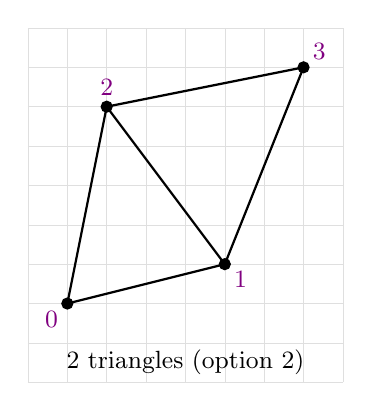
\begin{tikzpicture}
\draw[step=0.5cm,gray!25,very thin] (0.5,0) grid (4.5,4.5); 
\draw[black,fill=black] (1,1)   circle (2pt);
\draw[black,fill=black] (3,1.5)   circle (2pt);
\draw[black,fill=black] (1.5,3.5)   circle (2pt);
\draw[black,fill=black] (4,4)   circle (2pt);
\draw[-,thick] (1,1)--(3,1.5)--(4,4)--(1.5,3.5)--cycle;
\draw[-,thick] (3,1.5)--(1.5,3.5);
\node[] at (0.8,0.8) {\small \color{violet}0};
\node[] at (3.2,1.3) {\small \color{violet}1};
\node[] at (1.5,3.75) {\small \color{violet}2};
\node[] at (4.2,4.2) {\small \color{violet}3};
\node[] at (2.5,0.25) {\small 2 triangles (option 2)};
\end{tikzpicture}
\end{center}

When it comes to the quadrilateral, assuming a counterclockwise numbering, I can say that this quadrilaterals is then made of nodes 
{\color{violet}0}, {\color{violet}1},
{\color{violet}3} and {\color{violet}2}.
Note that I could also say it is made of nodes 
{\color{violet}3}, {\color{violet}2},
{\color{violet}0} and {\color{violet}1}.

Looking at the cases with 2 triangles I first need to label/number the triangles themselves:
\begin{center}
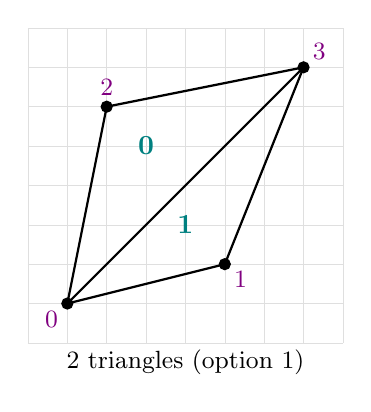
\begin{tikzpicture}
\draw[step=0.5cm,gray!25,very thin] (0.5,0.5) grid (4.5,4.5); 
\draw[black,fill=black] (1,1)   circle (2pt);
\draw[black,fill=black] (3,1.5)   circle (2pt);
\draw[black,fill=black] (1.5,3.5)   circle (2pt);
\draw[black,fill=black] (4,4)   circle (2pt);
\draw[-,thick] (1,1)--(3,1.5)--(4,4)--(1.5,3.5)--cycle;
\draw[-,thick] (1,1)--(4,4);
\node[] at (0.8,0.8) {\small \color{violet}0};
\node[] at (3.2,1.3) {\small \color{violet}1};
\node[] at (1.5,3.75) {\small \color{violet}2};
\node[] at (4.2,4.2) {\small \color{violet}3};
\node[] at (2,3) {\bf \color{teal}0};
\node[] at (2.5,2) {\bf \color{teal}1};
\node[] at (2.5,0.25) {\small 2 triangles (option 1)};
\end{tikzpicture}
\hspace{1cm}
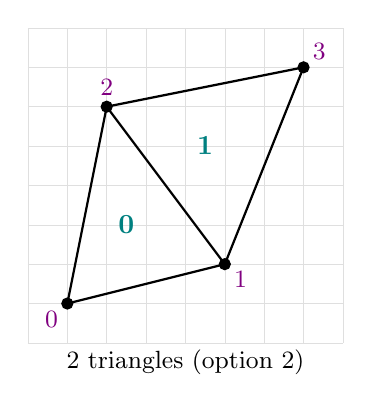
\begin{tikzpicture}
\draw[step=0.5cm,gray!25,very thin] (0.5,0.5) grid (4.5,4.5); 
\draw[black,fill=black] (1,1)   circle (2pt);
\draw[black,fill=black] (3,1.5)   circle (2pt);
\draw[black,fill=black] (1.5,3.5)   circle (2pt);
\draw[black,fill=black] (4,4)   circle (2pt);
\draw[-,thick] (1,1)--(3,1.5)--(4,4)--(1.5,3.5)--cycle;
\draw[-,thick] (3,1.5)--(1.5,3.5);
\node[] at (0.8,0.8) {\small \color{violet}0};
\node[] at (3.2,1.3) {\small \color{violet}1};
\node[] at (1.5,3.75) {\small \color{violet}2};
\node[] at (4.2,4.2) {\small \color{violet}3};
\node[] at (1.75,2) {\bf \color{teal}0};
\node[] at (2.75,3) {\bf \color{teal}1};
\node[] at (2.5,0.25) {\small 2 triangles (option 2)};
\end{tikzpicture}
\end{center}

In option 1, and still using a counterclockwise approach, triangle {\color{teal} 0} is made of nodes 
\{{\color{violet}0},{\color{violet}3},{\color{violet}2}\} and 
triangle {\color{teal} 1} is made of nodes 
\{{\color{violet}0},{\color{violet}1},{\color{violet}3}\}. 
In option 2, 
triangle {\color{teal} 0} is made of nodes 
\{{\color{violet}0},{\color{violet}1},{\color{violet}2}\} and 
triangle {\color{teal} 1} is made of nodes 
\{{\color{violet}1},{\color{violet}3},{\color{violet}2}\}. 

If I keep adding points, I will ultimately end up with a mesh which 
counts many quadrilaterals and/or triangles. In order to characterise this mesh, I need two numbers: $nel$, the number of elements (or cells) and $N$ the total number of vertices. However, this is not enough because I also need to know which vertex belongs to which element. 

Concretely, I need to store for each element a list of $m=3$ (triangles) or $m=4$ (quadrilaterals) numbers. The resulting array is often called the connectivity array. In FieldStone this array is always {\tt icon}, of size $m \times nel$.

In the cases above, $m=3$, $nel=2$, $N=4$ and 
\[
{\tt icon}_{\rm option\; 1}=
\left(
\begin{array}{cc}
{\color{violet}0}&{\color{violet}0}\\
{\color{violet}3}&{\color{violet}1}\\
{\color{violet}2}&{\color{violet}3}\\
\end{array}
\right)
\qquad
{\tt icon}_{\rm option\; 2}=
\left(
\begin{array}{cc}
{\color{violet}0}&{\color{violet}1}\\
{\color{violet}1}&{\color{violet}3}\\
{\color{violet}2}&{\color{violet}2}
\end{array}
\right)
\]
The way to understand these is as follows: for option 1,
\begin{itemize}
\item
icon[0,0]='the identity of node \#0 of element \#0' $\rightarrow$ {\color{violet}1}
\item
icon[1,0]='the identity of node \#1 of element \#0' $\rightarrow$ {\color{violet}4}
\item
icon[2,0]='the identity of node \#2 of element \#0' $\rightarrow$ {\color{violet}3}
\item
icon[0,1]='the identity of node \#0 of element \#1' $\rightarrow$ {\color{violet}1}
\item
icon[1,1]='the identity of node \#1 of element \#1' $\rightarrow$ {\color{violet}2}
\item
icon[2,1]='the identity of node \#2 of element \#1' $\rightarrow$ {\color{violet}4}
\end{itemize}

Finally, let us consider the following case:

\begin{center}
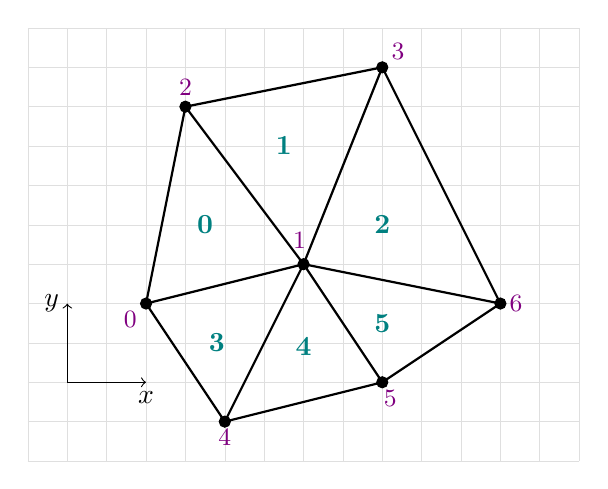
\begin{tikzpicture}
\draw[step=0.5cm,gray!25,very thin] (-0.5,-1) grid (6.5,4.5); 
\draw[black,fill=black] (1,1)   circle (2pt);
\draw[black,fill=black] (3,1.5)   circle (2pt);
\draw[black,fill=black] (1.5,3.5)   circle (2pt);
\draw[black,fill=black] (4,4)   circle (2pt);
\draw[black,fill=black] (5.5,1)   circle (2pt);
\draw[black,fill=black] (2.,-0.5)   circle (2pt);
\draw[black,fill=black] (4,0)   circle (2pt);

\draw[-,thick] (1,1)--(3,1.5)--(4,4)--(1.5,3.5)--cycle;
\draw[-,thick] (3,1.5)--(1.5,3.5);
\draw[-,thick] (3,1.5)--(5.5,1)--(4,4);
\draw[-,thick] (1,1)--(2,-0.5)--(4,0)--(5.5,1);
\draw[-,thick] (2,-0.5)--(3,1.5)--(4,0);
\node[] at (0.8,0.8) {\small \color{violet}0};
\node[] at (2.95,1.8) {\small \color{violet}1};
\node[] at (1.5,3.75) {\small \color{violet}2};
\node[] at (4.2,4.2) {\small \color{violet}3};
\node[] at (2,-0.7) {\small \color{violet}4};
\node[] at (4.1,-0.2) {\small \color{violet}5};
\node[] at (5.7,1) {\small \color{violet}6};

\node[] at (1.75,2) {\bf \color{teal}0};
\node[] at (2.75,3) {\bf \color{teal}1};
\node[] at (4,2) {\bf \color{teal}2};
\node[] at (1.9,0.5) {\bf \color{teal}3};
\node[] at (3,0.45) {\bf \color{teal}4};
\node[] at (4,0.75) {\bf \color{teal}5};


\draw[->] (0,0)--(1,0); 
\node[] at (1,-0.2) {$x$};
\draw[->] (0,0)--(0,1);
\node[] at (-0.2,1) {$y$};
\end{tikzpicture}
\end{center}
This mesh counts $nel=6$ elements/cells and $N=7$ points. 
The connectivity array is then of size $3\times 6$:
\[
{\tt icon}=
\left(
\begin{array}{cccccc}
{\color{violet}0}&{\color{violet}1}&{\color{violet}1}&{\color{violet}0}&{\color{violet}4}&{\color{violet}5}\\
{\color{violet}1}&{\color{violet}3}&{\color{violet}6}&{\color{violet}4}&{\color{violet}5}&{\color{violet}6}\\
{\color{violet}2}&{\color{violet}2}&{\color{violet}3}&{\color{violet}1}&{\color{violet}1}&{\color{violet}1}
\end{array}
\right)
\]
with 
\begin{align}
{\tt x}&=
\left(
\begin{array}{p{0.58cm}p{0.58cm}p{0.58cm}p{0.58cm}p{0.58cm}p{0.58cm}p{0.58cm}}
1 & 3 & 1.5 & 4 & 2 & 4 & 5.5
\end{array}
\right) \\
{\tt y}&=
\left(
\begin{array}{p{0.58cm}p{0.58cm}p{0.58cm}p{0.58cm}p{0.58cm}p{0.58cm}p{0.58cm}}
1 & 1.5 & 3.5 & 4 & -0.5 & 0 & 1
\end{array}
\right)
\end{align}

Let us then compute the barycenter coordinates of all triangles in arrays 
{\tt xb} and {\tt yb} of size $N=7$.
We need to loop over all triangles and for each compute the average of 
its nodes coordinates:
\begin{verbatim}
for iel in range(0,nel):
    xb[iel]=(x[icon[0,iel]]+x[icon[1,iel]]+x[icon[2,iel]])/3
    yb[iel]=(y[icon[0,iel]]+y[icon[1,iel]]+y[icon[2,iel]])/3
\end{verbatim}

The same concepts of course apply in 3D. In the case of tetrahedra then $m=4$ and in the case of hexahedra then $m=8$.

